% ---------------------------------------------------------------------
% Drop-in for Sec. VIII: the tightened per-run bound on the minimiser
% residual.  Replaces the cap RMS(E) + RMS(n) of (VIII.3)'s check.
%
% Figure: docs/fig_tight_rms.png, regenerated by
%     python analysis/failing_runs.py     DataSet/exp
%     python analysis/tight_rms_bound.py  docs/fig_tight_rms.png
% (the first writes the cache the second reads).
%
% Every constant's provenance is stated in Sec. 7: which numbers are
% a priori, which are campaign calibrations, and what breaks if the
% distinction is blurred.  Renumber (T.x) to match the host document.
% ---------------------------------------------------------------------

\documentclass[10pt]{article}
\usepackage[a4paper,margin=22mm]{geometry}
\usepackage{amsmath,amssymb,booktabs,graphicx,array}
\setlength{\parskip}{0.35em}\setlength{\parindent}{0pt}
\newcommand{\Mdot}{\dot M}
\newcommand{\rbar}{\bar\rho}
\newcommand{\rms}{\mathrm{RMS}}
\title{\vspace{-16mm}\textbf{A per-run bound on the minimiser residual,
tightened to the part of the model error the fit cannot absorb}
\vspace{-3mm}}
\date{\small drop-in for Sec.~VIII; figure \texttt{fig\_tight\_rms.png}}
\begin{document}\maketitle

\begin{figure}[t]
\centering
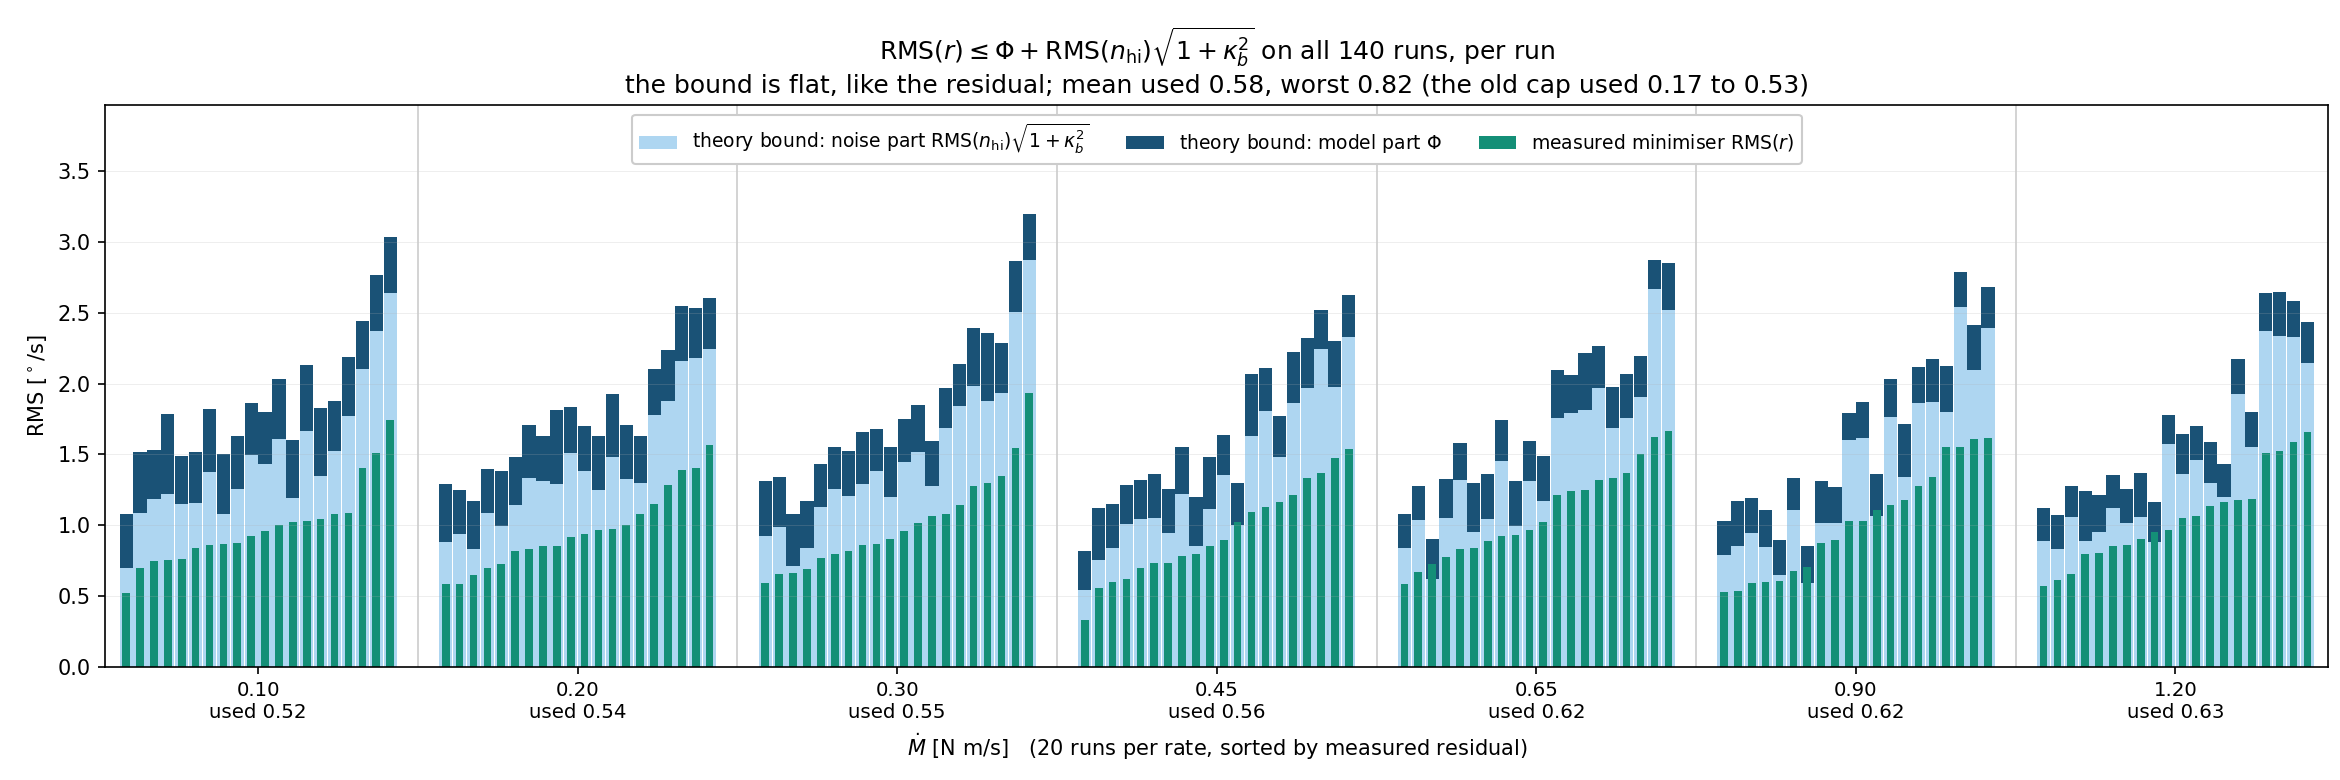
\includegraphics[width=\linewidth]{fig_tight_rms.png}
\caption{The bound (T.6) against the measured minimiser residual, every
run drawn individually: $20$ runs per rate, sorted within each rate by
the measured residual. Each light bar is the noise part of the bound,
$\rms(n_{\rm hi})\sqrt{1+\kappa_b^2}$, built from that run's own
measured content above $5$~Hz; the dark segment on top is the model
part $\Phi$; the green bar is the measured residual $\rms(\hat r)$. The
bound holds on all $140$ runs, with a mean used fraction of $0.58$ and
a worst of $0.82$, and it is flat across the rates --- like the
residual, and unlike the old cap, whose used fraction ran $0.17$ to
$0.53$.}
\label{fig:tight-rms}
\end{figure}

\section{Notation}

All quantities refer to one run's post-onset window unless stated. The
table is complete; symbols not listed here do not appear.

\begin{center}\small
\begin{tabular}{@{}>{$}l<{$}p{121mm}@{}}
\toprule
\tau & time since the identified onset, $\tau\in[0,\tau_{\rm end}]$ [s]\\
\tau_{\rm end} & window length; $x = C_2\tau_{\rm end}$ is its
  dimensionless form\\
\tau_i,\ N & the $N$ sample instants $0=\tau_1<\dots<\tau_N=
  \tau_{\rm end}$ (logging period $T_s\approx10$~ms)\\
y_i & measured roll/pitch rate at $\tau_i$, from the flight IMU
  [rad/s]\\
\omega_{\rm nom}(\tau) & nominal response
  $C_1(\cosh C_2\tau - 1) + C$ [rad/s]\\
C_1,\ C_2,\ C & amplitude $C_1 = K\Mdot$, exponent
  $C_2 = \sqrt{Wz_{CoM}/J_P}$, pre-onset baseline $C$\\
K,\ \Mdot & calibrated gain $K = 1/(Wz_{CoM})$ [1/(N\,m\,s)] and
  commanded ramp rate [N\,m/s]\\
W,\ z_{CoM},\ J_P & weight [N], CoM height [m], pivot-axis inertia
  [kg\,m$^2$]; $J_P = 1/(KC_2^2)$\\
e_\omega(\tau) & deviation of the true (noise-free) rate from
  $\omega_{\rm nom}$ [rad/s]\\
n_i & in-window disturbance: everything in $y$ that is neither
  $\omega_{\rm nom}$ nor $e_\omega$ [rad/s]\\
u_i & regressor $u_i = \cosh C_2\tau_i - 1$;\quad
  $\tilde u_i = u_i - \bar u$ its centred form\\
V,\ A,\ P & fitted family's span $V=\operatorname{span}\{u,\mathbf 1\}$;
  $A = [\,u\ \ \mathbf 1\,]$; projector $P = A(A^\top\! A)^{-1}A^\top$,
  in closed form $P_{ij} = 1/N + \tilde u_i\tilde u_j/\sum_k\tilde
  u_k^2$\\
\hat r & minimiser residual $\hat r = (I-P)\,y$: the per-run fit with
  $C_2$ pinned and $(C_1, C)$ free is exactly this projection\\
\rho(s) & deviation forcing at time $s$: the gravity remainder
  $Wz_{CoM}(\sin\varphi - \varphi)$ plus the ground-effect terms,
  evaluated on the true trajectory [N\,m]\\
\rbar & a priori pointwise bound $|\rho(s)|\le\rbar$ from the
  $10^\circ$ box, as in (93) [N\,m]\\
k_j & kernel column: response of $e_\omega$ at the samples to a unit
  impulse of $\rho$ at $\tau_j$, i.e.\
  $k_j(\tau_i) = \Delta s_j\cosh\!\big(C_2(\tau_i-\tau_j)\big)/J_P$ for
  $\tau_i\ge\tau_j$, else $0$; $\Delta s_j$ the trapezoidal quadrature
  weight [s]\\
\Phi & a priori bound on $\rms\big((I-P)\,e_\omega\big)$, eq.~(T.4)
  [rad/s, reported in $^\circ$/s]\\
E(\tau) & the pointwise envelope of (93),
  $E = \rbar\sinh(C_2\tau)/(J_PC_2)$; note
  $E(\tau) = \rbar\sum_j |k_j(\tau)|$ --- the same kernel without the
  projection\\
n_{\rm hi} & the part of $\hat r$ above $f_c = 5$~Hz; attributable to
  disturbance because the family and $e_\omega$ are smooth on the
  window scale\\
\kappa & spectral shape ratio $\rms({<}f_c)/\rms({>}f_c)$ of a
  disturbance record\\
\kappa_q & $\kappa$ measured on the run's quiet stretch of equal
  length, ending at the excitation start\\
\kappa_{\rm imp} & in-window implied ratio
  $\sqrt{\rms(\hat r)^2 - \rms(n_{\rm hi})^2}\,/\,\rms(n_{\rm hi})$\\
s_{\rm med},\ \kappa_b & median in-window enhancement
  $s_{\rm med} = \operatorname{med}(\kappa_{\rm imp}/\kappa_q)$;
  campaign constant $\kappa_b = s_{\rm med}\,\max_{\rm runs}\kappa_q$\\
\rms(v) & $\sqrt{\tfrac1N\sum_i v_i^2}$ for sampled $v$ (uniform grid;
  trapezoidal end weights where integrals are quoted)\\
\bottomrule
\end{tabular}
\end{center}

\section{The residual sees only what the family cannot absorb}

The per-run fit holds $C_2$ at its physical value and minimises over
$(C_1, C)$, which is linear least squares on $A$: the fitted curve is
$Py$ and the residual is $\hat r = (I-P)y$. The record decomposes as
$y = \omega_{\rm nom} + e_\omega + n$, and $\omega_{\rm nom}\in V$
exactly (it is $C_1 u + (C_1\cdot 0 + C)\mathbf 1$ evaluated at the same
pinned $C_2$), so $(I-P)\,\omega_{\rm nom} = 0$ and
\begin{equation}
  \hat r \;=\; (I-P)\,(e_\omega + n).
  \tag{T.1}
\end{equation}
Hence
\begin{equation}
  \rms(\hat r)\;\le\;\rms\big((I-P)e_\omega\big) +
  \rms\big((I-P)n\big),
  \tag{T.2}
\end{equation}
and this is where the old cap gave ground: it bounded the first term by
$\rms(e_\omega)\le\rms(E)$, the size of the deviation itself. But the
minimiser absorbs whatever part of $e_\omega$ lies in $V$, and most of
it does. That is not an accident of the data --- it is structural.
$e_\omega$ is built from the kernel columns, and a shifted cosh splits
as
\begin{equation}
  \cosh\!\big(C_2(\tau - s)\big)
  = \cosh(C_2 s)\,\cosh(C_2\tau) - \sinh(C_2 s)\,\sinh(C_2\tau),
  \tag{T.3}
\end{equation}
whose first part is $u + \mathbf 1\in V$ \emph{exactly}. What survives
the projection is only the $\sinh(C_2\tau)$ part, weighted by
$\sinh(C_2 s)$ --- small for impulses early in the window --- plus the
truncation of the kernel before its impulse time. Norm-weighted over
the columns, the family absorbs $68$ to $91\%$ of the kernel
($79.7\%$ in the median across runs) before any property of $\rho$ is
used.

\section{The model term $\Phi$}

By Duhamel on the deviation dynamics
$J_P\ddot e_\varphi = Wz_{CoM}\,e_\varphi + \rho$ (with
$e_\varphi(0)=\dot e_\varphi(0)=0$; $e_\omega = \dot e_\varphi$), the
sampled deviation is $e_\omega = \sum_j \rho(\tau_j)\,k_j$ to
quadrature accuracy. Linearity of $I-P$, the triangle inequality
applied pointwise, and $|\rho|\le\rbar$ give
\begin{equation}
  \big|\big[(I-P)\,e_\omega\big]_i\big|
  \;\le\; \rbar\sum_j\big|\big[(I-P)\,k_j\big]_i\big|
  \qquad\Longrightarrow\qquad
  \rms\big((I-P)e_\omega\big)\;\le\;\Phi
  \;=\;\rbar\,\Big\|\textstyle\sum_j\big|(I-P)k_j\big|\Big\|_{\rms},
  \tag{T.4}
\end{equation}
computable a priori from $(C_2, J_P, \rbar)$ and the sample grid alone.
Without the projection the same construction returns exactly the old
envelope, $\rbar\sum_j|k_j(\tau)| = E(\tau)$, so the ratio
$\rms(E)/\Phi$ isolates what absorption is worth: a factor $12$ at
$\Mdot=0.10$~N\,m/s falling to $4$ at $1.20$, with
$\Phi = 0.40$ down to $0.26^\circ$/s.

Both the representation and the bound were verified on the exact
nonlinear tip-over: the kernel sum reconstructs $e_\omega$ to
$3\times10^{-4}\,{}^\circ$/s, and the realised
$\rms\big((I-P)e_\omega\big)$ is $0.065$--$0.078^\circ$/s across the
rates --- inside $\Phi$ with a factor $4$ to $5$ to spare, of which
about $2$ is $\rbar$ against the realised $|\rho|$ and about $2$ is the
sign coherence the triangle step discards.

\section{The noise term}

Projections contract, so $\rms\big((I-P)n\big)\le\rms(n)$, and the task
is an estimate of $\rms(n)$ that does not use the residual being
bounded. Its high-frequency part needs no estimation:
above $f_c = 5$~Hz the family and $e_\omega$ are smooth on the window
scale and can contribute nothing --- and by (T.4) their total
contribution anywhere is at most $\Phi$ --- so $n_{\rm hi}$ is measured
directly from the record. The low-frequency part is extended from it by
a spectral shape ratio: $\rms(n) = \rms(n_{\rm hi})\sqrt{1+\kappa^2}$
for the in-window $\kappa$.

The campaign fixes $\kappa$'s scale but not its per-run value. On the
$113$ runs with a quiet stretch of equal window length,
$\kappa_q$ runs $0.15$ (p10) to $1.31$ (max), median $0.37$, and,
decisively, $\kappa_q$ does not predict the in-window ratio run by run
(Pearson $r = 0.04$, $p = 0.70$). A per-run noise model is therefore
not available, and the bound uses the campaign envelope --- measured
entirely outside the windows it will be tested on:
\begin{equation}
  \kappa_b \;=\; \max_{\rm runs}\kappa_q \;=\; 1.31,
  \qquad \sqrt{1+\kappa_b^2} \;=\; 1.65.
  \tag{T.5}
\end{equation}

\section{The bound, on the campaign}

\begin{equation}
  \boxed{\;\rms(\hat r)\;\le\;\Phi
  \;+\;\rms(n_{\rm hi})\,\sqrt{1+\kappa_b^2}\;}
  \tag{T.6}
\end{equation}

per run, with $\Phi$ from (T.4) and the run's own measured
$n_{\rm hi}$. On the $140$ runs (means over the $20$ at each rate):

\begin{center}\small
\begin{tabular}{@{}rrrrrrrrr@{}}
\toprule
$\Mdot$ & $\Phi$ & $\rms(E)$ & $\rms(E)/\Phi$ & cap (T.6) & old cap &
$\rms(\hat r)$ & used & old used\\
N\,m/s & $^\circ$/s & $^\circ$/s & & $^\circ$/s & $^\circ$/s &
$^\circ$/s & & \\
\midrule
$0.10$ & $0.403$ & $4.876$ & $12$ & $1.87$ & $5.77$ & $0.987$ & $0.53$ & $0.17$\\
$0.20$ & $0.364$ & $2.934$ & $8$  & $1.78$ & $3.79$ & $0.964$ & $0.54$ & $0.25$\\
$0.30$ & $0.341$ & $2.308$ & $7$  & $1.84$ & $3.22$ & $1.014$ & $0.55$ & $0.32$\\
$0.45$ & $0.320$ & $1.892$ & $6$  & $1.67$ & $2.71$ & $0.947$ & $0.57$ & $0.35$\\
$0.65$ & $0.295$ & $1.516$ & $5$  & $1.78$ & $2.42$ & $1.084$ & $0.61$ & $0.45$\\
$0.90$ & $0.274$ & $1.260$ & $5$  & $1.66$ & $2.10$ & $1.023$ & $0.62$ & $0.49$\\
$1.20$ & $0.262$ & $1.120$ & $4$  & $1.68$ & $1.98$ & $1.052$ & $0.63$ & $0.53$\\
\bottomrule
\end{tabular}
\end{center}

It holds on every run --- per-run used fraction p10 $0.49$, median
$0.56$, p90 $0.68$, worst $0.82$ --- it is below the old cap at every
rate, and it is \emph{flat}: the cap runs $1.66$ to $1.87^\circ$/s
across a twelvefold change in ramp rate, matching the flat residual,
where the old cap fell $5.77$ to $1.98$.

Little of the remaining width is removable within this form. The
binding run fixes the smallest admissible cap factor at $1.28$ (against
the $1.65$ in use), and even at that untenable limit --- it is set by
the very run it must cover --- the mean used fraction only reaches
$0.70$. The distance from $0.58$ to that ceiling is the price of
covering the worst spectral shape in the campaign with one constant.

\section{What the bound says, and what it cannot}

Applying (T.4) to (T.1) two-sidedly gives
\begin{equation}
  \big|\,\rms(\hat r) - \rms\big((I-P)n\big)\,\big| \;\le\; \Phi ,
  \tag{T.7}
\end{equation}
so the residual \emph{is} the projected disturbance to within
$0.26$--$0.40^\circ$/s. That is the flatness of Fig.~\ref{fig:tight-rms}
read as a theorem: the residual does not depend on $\Mdot$ because the
disturbance floor does not, and the model error, whose bound does fall
with the rate, is capped at a third of the residual's size in the
median --- $11\%$ of its power. The same statement fixes the limit of
this check:
a residual test can confirm $\rho$'s contribution is below $\Phi$, but
it cannot resolve $\rho$ inside the disturbance floor. The instrument
that tests $\rho$ is the forward check of (108), which propagates each
perturbation along the measured trajectory and is not noise-limited.

\section{Provenance of every constant}

$C_2$, $K$, $J_P$ are the per-configuration calibration constants,
fixed before this analysis. $\rbar$ is a priori from the $10^\circ$
box, as in (93). The kernel, the projector and hence $\Phi$ follow
from those alone: the model part of (T.6) uses nothing measured in the
window. The noise part uses one campaign scalar,
$\max\kappa_q = 1.31$, from the quiet stretches only --- the bound is
built entirely from data outside the windows it is tested on.

One caveat is measured and stated rather than hidden. The in-window
spectra are heavier at low frequency than the quiet ones ---
$s_{\rm med} = \operatorname{med}(\kappa_{\rm imp}/\kappa_q) = 1.60$,
which is what pivoting on one gear edge adds --- so on $5$ of the
$140$ runs the residual exceeds the noise term of (T.6) alone, and it
is $\Phi$'s margin that covers them. A reader who wants the noise term
safe by construction can take
$\kappa_b = s_{\rm med}\times1.31 = 2.09$: that variant also holds on
all $140$ runs, at a mean used fraction of $0.44$, and prices the
in-window enhancement at about $0.6^\circ$/s of cap. The tight version
is reported as the result and the conservative one as the price of
removing its caveat.

\end{document}
